We begin our empirical analysis by estimating the causal effect of app access on household electricity consumption, addressing our first research question: how persistent are feedback-induced savings from continuous smartphone feedback? Given the staggered rollout across three tranches, we estimate dynamic treatment effects following \citet{sunEstimatingDynamicTreatment2021}:
\[
y_{it} = \sum_{k \neq -1} \beta_k \cdot \mathbb{1}\{t - G_i = k\} + \alpha_i + \delta_t + \varepsilon_{it},
\]
where $y_{it}$ is household $i$'s daily electricity consumption (kWh, aggregated from 15-minute smart meter data), $G_i$ denotes app access timing, $\beta_k$ traces effects relative to the $k=-1$ pre-treatment reference, $\alpha_i$ absorbs time-invariant household differences, and $\delta_t$ controls common shocks (weekly or daily fixed effects). Standard errors are clustered at the household level.

Table \ref{table:main_results} presents the main results. Across specifications, we observe a consistent reduction in electricity consumption following access to the application (columns 1--3). In the baseline specification (column 1), the TWFE estimate indicates a decrease of 0.47 kWh per household per day (SE = 0.206, $p = 0.023$). The corresponding Sun--Abraham estimate is similar in magnitude ($-0.45$ kWh, SE = 0.294, $p = 0.128$), suggesting that accounting for staggered treatment timing and heterogeneous effects does not materially alter the point estimate, although statistical precision is reduced. Including weekly fixed effects yields nearly identical results, with estimated reductions of 0.46--0.47 kWh (column 3). In proportional terms, this corresponds to a reduction of approximately 4.7\% in electricity consumption.\footnote{The percentage effect is based on a log-linear specification using $\log(\text{consumption})$ as the dependent variable.} 

From a behavioral perspective, these results are consistent with a salience-based mechanism: by continuously providing feedback, the application makes electricity consumption more cognitively accessible, thereby increasing the likelihood that households adjust their behavior. The persistence of the effect suggests that this is not merely a short-lived attention shock. 

To further investigate the underlying behavioral adjustments, we decompose total consumption into flexible (hours 7--22) and non-flexible (hours 23--6) components. The reduction in electricity use is primarily driven by flexible consumption, where households have greater scope for behavioral adaptation. In this domain, the estimated treatment effect ranges from 0.31 to 0.33 kWh (e.g., column 4: $-0.31$ kWh, SE = 0.156, $p = 0.048$), indicating economically meaningful reductions. In contrast, the effect on non-flexible consumption is smaller (approximately $-0.14$ to $-0.15$ kWh; column 5: $p = 0.082$) and only weakly statistically significant.



\begin{table}[htbp]\centering
\caption{Treatment Effects on Electricity Consumption}
\label{table:main_results}
\begin{threeparttable}
\begin{tabular}{lccccc}
\toprule
 & 1 & 2 & 3 & 4 & 5 \\
\midrule

\textbf{TWFE} \\
Treatment effect 
& -0.4685** 
& -0.0187** 
& -0.4612** 
& -0.3107** 
& -0.1526* \\
& (0.2061) 
& (0.0086) 
& (0.2059) 
& (0.1562) 
& (0.0784) \\

\addlinespace
\textbf{Sun--Abraham ATT} \\
ATT 
& -0.4500 
& --- 
& -0.4736** 
& -0.3323* 
& -0.1424 \\
& (0.2938) 
& --- 
& (0.2343) 
& (0.1730) 
& (0.0939) \\

\midrule
Observations 
& 354,121 
& 8,287,525 
& 354,121 
& 354,096 
& 354,121 \\

Household FE & Yes & Yes & Yes & Yes & Yes \\
Time FE & Day & Day & Week & Week & Week \\

\bottomrule
\end{tabular}

\begin{tablenotes}
\footnotesize
\item Notes: The table reports treatment effects on electricity consumption (kWh). 
TWFE estimates are obtained from two-way fixed effects regressions. Sun--Abraham estimates report the aggregated ATT from staggered difference-in-differences models. 
All standard errors are clustered at the household level. 
Significance levels: ** $p<0.05$, * $p<0.10$.
\end{tablenotes}

\end{threeparttable}
\end{table}


\subsection{Effects over time}

We begin by examining the overall effect of app access on household electricity consumption. The dynamic difference-in-differences estimates indicate a consistent reduction in consumption following treatment. In the early post-treatment period, the effect becomes statistically significant after approximately two weeks. For instance, in week 2, consumption decreases by 0.365 kWh (SE = 0.175, $p = 0.037$), and the effect strengthens in subsequent weeks. By week 3, the estimated reduction amounts to 0.572 kWh (SE = 0.184, $p = 0.002$), and reaches 0.978 kWh in week 11 (SE = 0.324, $p = 0.003$). 

Over time, the effect stabilizes at a lower but still economically meaningful level. In later periods, the estimates remain negative, and the pooled effect beyond week 50 is approximately 0.55 kWh, indicating persistent reductions in electricity consumption. The absence of significant pre-treatment effects supports the identifying assumption of parallel trends.

To better understand the underlying behavioral adjustments, we decompose total consumption into flexible and non-flexible components. The reduction in electricity use is primarily driven by flexible consumption, where households have greater scope to adjust their behavior. For example, in week 3, flexible consumption decreases by 0.476 kWh (SE = 0.154, $p = 0.002$), closely mirroring the total effect. Similarly, in week 11, the reduction in flexible consumption amounts to 0.759 kWh (SE = 0.236, $p = 0.001$). 

In contrast, the effect on non-flexible consumption is substantially smaller and only occasionally statistically significant. For instance, in week 3, non-flexible consumption decreases by 0.096 kWh (SE = 0.057, $p = 0.093$), and in week 11 by 0.218 kWh (SE = 0.119, $p = 0.066$). Overall, these estimates suggest that households adjust their behavior primarily along margins where consumption is discretionary, while essential usage remains largely unchanged.

Taken together, the results indicate that real-time feedback induces persistent reductions in electricity consumption, driven mainly by adjustments in flexible usage. The dynamic pattern—characterized by a gradual increase in treatment effects followed by stabilization—is consistent with a behavioral mechanism in which repeated exposure to consumption information increases salience and facilitates sustained behavioral change.

\begin{figure}
    \centering
    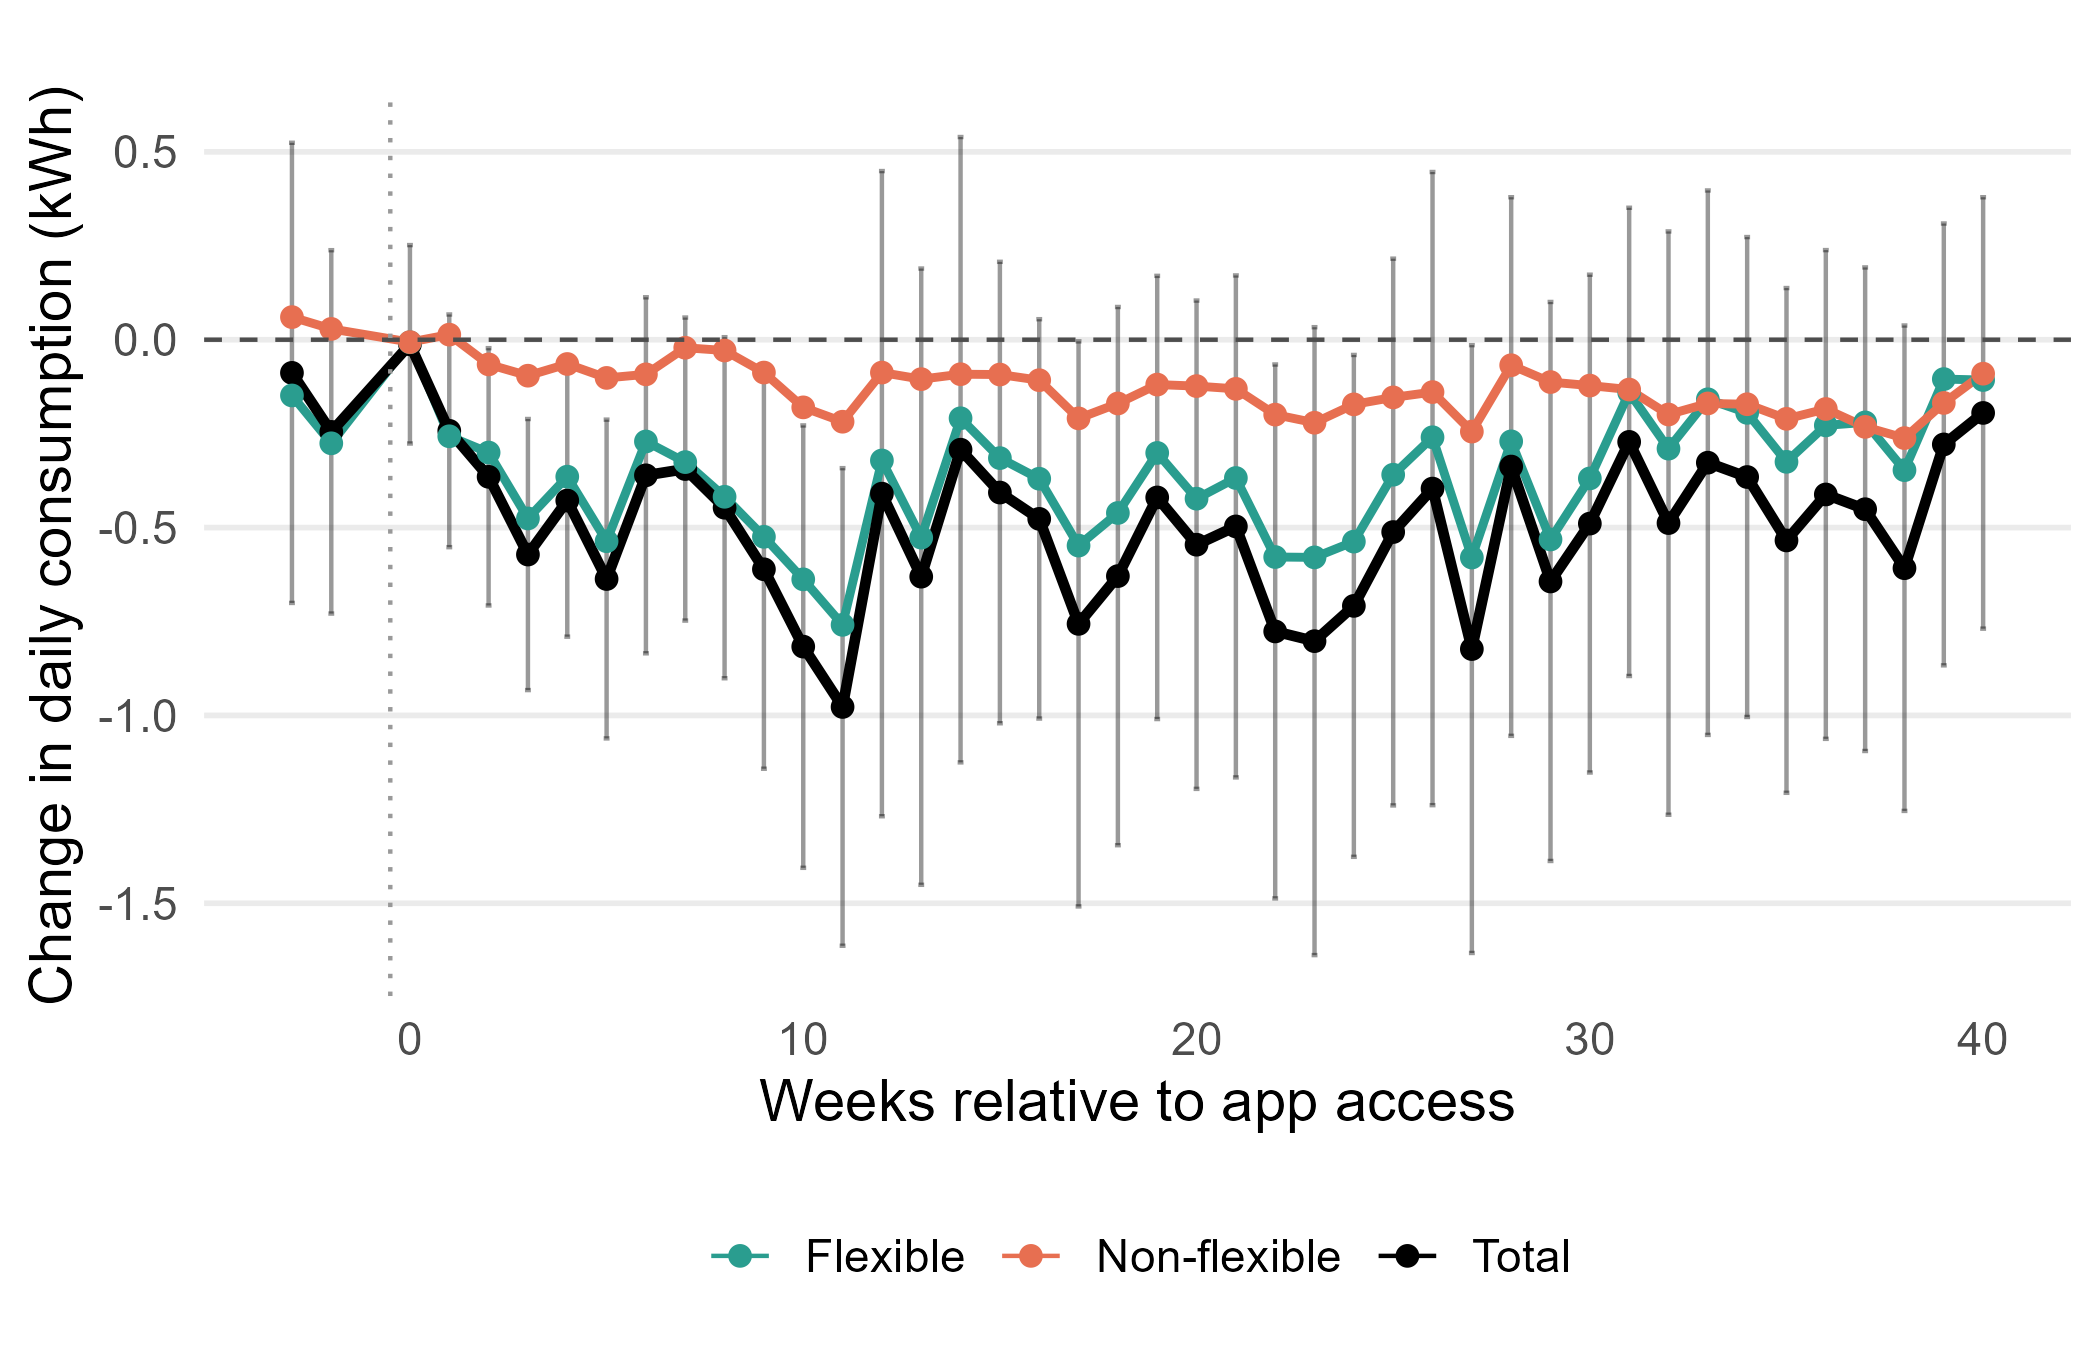
\includegraphics[width=1\linewidth]{paper/figures/event_study_consumption.png}
    \caption{Caption}
    \label{fig:placeholder}
\end{figure}